%\documentclass[preprint,12pt,authoryear]{elsarticle}
%% \documentclass[final,1p,times,authoryear]{elsarticle}
%% \documentclass[final,1p,times,twocolumn,authoryear]{elsarticle}
%% \documentclass[final,3p,times,authoryear]{elsarticle}
\documentclass[final,3p,times,twocolumn,authoryear]{elsarticle}
%% \documentclass[final,5p,times,authoryear]{elsarticle}
%% \documentclass[final,5p,times,twocolumn,authoryear]{elsarticle}

\usepackage{amssymb}

\journal{Indonesian Journal of Science \& Technology}

\begin{document}

\begin{frontmatter}

%% Title, authors and addresses

%% use the tnoteref command within \title for footnotes;
%% use the tnotetext command for theassociated footnote;
%% use the fnref command within \author or \address for footnotes;
%% use the fntext command for theassociated footnote;
%% use the corref command within \author for corresponding author footnotes;
%% use the cortext command for theassociated footnote;
%% use the ead command for the email address,
%% and the form \ead[url] for the home page:
 \title{Judul Artikel dari Jurnal}
 \tnotetext[label1]{}
 \author{Rolly Maulana Awangga\corref{cor1}\fnref{label2}}
 \ead{awangga@poltekpos.ac.id}
 \ead[url]{home page}
 \fntext[label2]{}
 \cortext[cor1]{}
 \address{Address\fnref{label3}}
 \fntext[label3]{}

%%%\title{Judul Artikel}

%% use optional labels to link authors explicitly to addresses:
%% \author[label1,label2]{}
%% \address[label1]{}
%% \address[label2]{}

%\author{}

%\address{}
	\begin{abstract}


A well-prepared abstract enables the reader to identify the basic content of a document quickly and accurately, to determine its relevance to their interests, and thus to decide whether to read the document in its entirety. The Abstract should be informative and completely self-explanatory, provide a clear statement of the problem, the proposed approach or solution, and point out major findings and conclusions. The Abstract should be 100 to 200 words in length. The abstract should be written in the past tense. Standard nomenclature should be used and abbreviations should be avoided. No literature should be cited. The keyword list provides the opportunity to add keywords, used by the indexing and abstracting services, in addition to those already present in the title. Judicious use of keywords may increase the ease with which interested parties can locate our article.

\end{abstract}

\begin{keyword}
	kata kunci \sep kunci kata
	%% keywords here, in the form: keyword \sep keyword

	%% PACS codes here, in the form: \PACS code \sep code

	%% MSC codes here, in the form: \MSC code \sep code
	%% or \MSC[2008] code \sep code (2000 is the default)
\end{keyword}

\end{frontmatter}

%% \linenumbers

%% main text
\section{Introduction}
\label{Introduction}
Ceritanya ini paragraph pertama\cite{awangga2018ontology}.The main text format consists of a flat left-right columns on A4 paper (quarto)\cite{armiati2018national}. The margin text from the left, right, top, and bottom 3 cm\cite{setyawan2018comparison}. The manuscript is written in Microsoft Word\cite{pane2018analysis}, single space, Arial 10pt and maximum 12 pages\cite{awangga2019implementation}, which can be downloaded at the website: http://www.telkomnika.ee.uad.ac.id\cite{awangga2017colenak}.

ini merupakan paragraph kedua cuy etc\cite{awangga2019kafa}. Indexing and abstracting services depend on the accuracy of the title\cite{awangga2019ontology}, extracting from it keywords useful in cross-referencing and computer searching\cite{maulani2018analysis}. An improperly titled paper may never reach the audience for which it was intended\cite{harani2018improving}, so be specific\cite{awangga2018k}.

Ini paragraph ketiga\cite{yulita2018feature}.The Introduction should provide a clear background\cite{pane2019rfid}, a clear statement of the problem, the relevant literature on the subject, the proposed approach or solution, and the new value of research which it is innovation. It should be understandable to colleagues from a broad range of scientific disciplines. Organization and citation of the bibliography are made in Vancouver style in sign, and so on. The terms in foreign languages are written italic (italic)\cite{awangga2018sampeu}. The text should be divided into sections, each with a separate heading and numbered consecutively. The section/subsection headings should be typed on a separate line, e.g., 1. Introduction . Authors are suggested to present their articles in the section structure: Introduction - the comprehensive theoretical basis and/or the Proposed Method/Algorithm - Research Method - Results and Discussion – Conclusion\cite{pane2018qualitative}.

Paragraph ke empat . Literature review that has been done author used in the chapter `Introduction' to explain the difference of the manuscript with other papers, that it is innovative, it are used in the chapter `Research Method' to describe the step of research and used in the chapter `Results and Discussion' to support the analysis of the results . If the manuscript was written really have high originality, which proposed a new method or algorithm, the additional chapter after the `Introduction' chapter and before the `Research Method' chapter can be added to explain briefly the theory and/or the proposed method/algorithm\cite{setyawan2018analysis}.

\section{Related Works}
\label{RelatedWorks}
This is related works

\section{Research Method}
\label{ResearchMethod}
Explaining research chronological, including research design, research procedure (in the form of algorithms, Pseudocode or other), how to test and data acquisition. The description of the course of research should be supported references, so the explanation can be accepted scientifically.
\par
Tables \ref{contohtabel} and Figures \ref{contohgambar} are presented center, as shown below and cited in the manuscript.\\

\begin{table}[ht]
\caption{The Performance of ...}
\centering
\begin{tabular}{lcr}
\hline
Variable & Speed (rpm) & Power (kW) \\
\hline
x & 10 & 8.6 \\
y & 15 & 12.4 \\
z & 20 & 15.3 \\
\hline
\end{tabular}
\label{contohtabel}
\end{table}

\begin{figure}[ht]
\centering
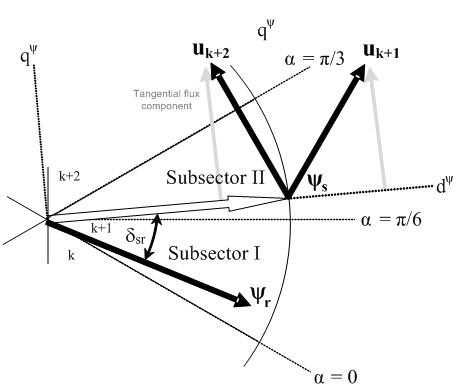
\includegraphics[scale=0.5]{figures/figure1}
\caption{Effects of selecting different switching under dynamic condition}
\label{contohgambar}
\end{figure}

\section{Result and Analysis}
\label{ResultAnalysis}
In this section, it is explained the results of research and at the same time is given the comprehensive discussion. Results can be presented in figures, graphs, tables and others that make the reader understand easily. The discussion can be made in several sub-chapters.

\subsection{Equations}
Equations should be placed at the center of the line and provided consecutively with equation numbers in parentheses flushed to the right margin, as in (1). The use of Microsoft Equation Editor or MathType is preferred.

\begin{equation}
E_v - E = \frac{\hbar}{2.m}(k_x^2 + k_y^2)
\end{equation}

All symbols that have not been mentioned in the equation should be explained in the following text.

\subsection{Citations}
Proper citation of other works should be made to avoid plagiarism. When referring to a reference item, please use the reference number as in or , Arulmozhiyal, Zhang, Yinhai, lamport, knuth for multiple references. The use of should be employed for any reference citation at the beginning of sentence. For any reference with more than 3 or more authors, only the first author is to be written followed by et al (e.g. in ).  Examples of reference items of different categories shown in the References section. Each items in the references section should be typed using 9pt font size.


\section{Conclusion}
\label{Conclusion}
Provide a statement that what is expected, as stated in the `Introduction' chapter can ultimately result in `Results and Discussion' chapter, so there is compatibility. Moreover, it can also be added the prospect of the development of research results and application prospects of further studies into the next (based on result and discussion).

\section{Acknowledgement}
\label{Ack}
The acknowledgment section is optional. The funding source of the research can be put here.



%% The Appendices part is started with the command \appendix;
%% appendix sections are then done as normal sections
%% \appendix

\section{REFERENCES}
\label{references}


\bibliographystyle{elsarticle-harv} 
\bibliography{references}

\end{document}

\endinput

